\documentclass[]{standalone}
\usepackage{amsmath, amssymb, amsfonts}
\usepackage{tudscrcolor} 
\usepackage{pgfplots}
\usepgfplotslibrary{fillbetween} 
\pgfplotsset{
  compat=1.10,% mit writeLaTeX bisher noch nicht möglich
  flaeche/.style={draw=none,fill=black,fill opacity=0.2},
  every axis/.append style={
  	axis x line=middle,    % put the x axis in the middle
  	axis y line=middle,    % put the y axis in the middle
  	axis line style={->},  % arrows on the axis
  }
}

\renewcommand{\Re}{\mathrm{Re}}
\renewcommand{\Im}{\mathrm{Im}}

\usepackage{opensans}
\usepackage{sfmath}

\begin{document} 

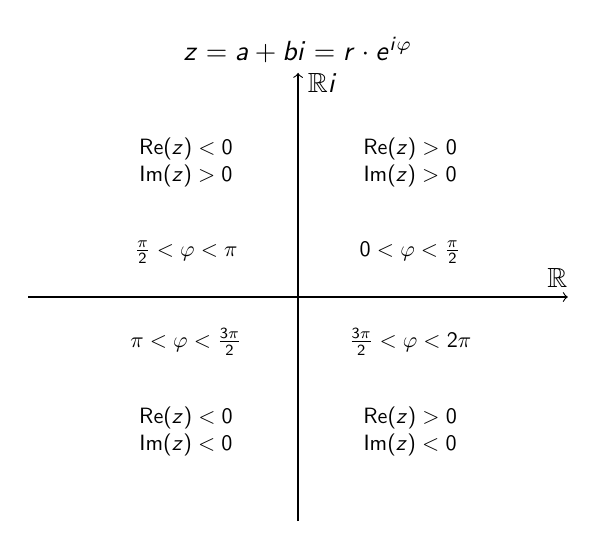
\begin{tikzpicture} 
	\begin{axis}[%
		xmin = -10,
		xmax =  10,
		ymin = -10,
		ymax =  10,
		axis equal,
		ticks=none,
		grid=none,
		xlabel=$\mathbb{R}$,
		xlabel style={below, anchor=south east,inner xsep=0pt},
		ylabel=$\mathbb{R}i$,
		ylabel style={above,anchor=north west,inner ysep=0pt},
%		xtick = {4.5},
%		xticklabels = {$a$},
%		tick style={ultra thick, black}, 
%		ytick = {7.79},
%		yticklabels= {$b$}, 
	]
	
		\node[align=center, scale=0.8] at (axis cs: 5,6) {$\Re(z) > 0$ \\ $\Im(z) > 0$};
		\node[align=center, scale=0.8] at (axis cs: 5,2) {$0 < \varphi < \frac \pi 2$};	
		
		\node[align=center, scale=0.8] at (axis cs: -5,6) {$\Re(z) < 0$ \\ $\Im(z) > 0$};
		\node[align=center, scale=0.8] at (axis cs: -5,2) {$\frac \pi 2 < \varphi < \pi$};
		
		\node[align=center, scale=0.8] at (axis cs: -5,-6) {$\Re(z) < 0$ \\ $\Im(z) < 0$};
		\node[align=center, scale=0.8] at (axis cs: -5,-2) {$\pi < \varphi < \frac{3\pi}{2}$};
		
		\node[align=center, scale=0.8] at (axis cs: 5,-6) {$\Re(z) > 0$ \\ $\Im(z) < 0$};
		\node[align=center, scale=0.8] at (axis cs: 5,-2) {$\frac{3\pi}{2} < \varphi < 2\pi$};
		
		
	\end{axis} 

	\node[above,font=\bfseries] at (current bounding box.north) {$z = a + bi = r \cdot e^{i \varphi}$};
	
\end{tikzpicture} 






\end{document}